\documentclass[UTF8]{ctexart}
\usepackage{xcolor}
\usepackage{enumerate}
\usepackage{graphicx}
\usepackage{geometry}
\usepackage{graphicx} %插入图片的宏包
\usepackage{float} %设置图片浮动位置的宏包
\usepackage{subfigure} 
\usepackage[colorlinks,linkcolor=blue]{hyperref}
%插入多图时用子图显示的宏包
\usepackage{listings}
\lstset{ %
    language=python,                % the language of the code
    basicstyle=\footnotesize,           % the size of the fonts that are used for the code
    numbers=left,                   % where to put the line-numbers
    numberstyle=\tiny\color{gray},  % the style that is used for the line-numbers
    stepnumber=2,                   % the step between two line-numbers. If it's 1, each line 
                                    % will be numbered
    numbersep=5pt,                  % how far the line-numbers are from the code
    backgroundcolor=\color{white},      % choose the background color. You must add \usepackage{color}
    showspaces=false,               % show spaces adding particular underscores
    showstringspaces=false,         % underline spaces within strings
    showtabs=false,                 % show tabs within strings adding particular underscores
    frame=single,                   % adds a frame around the code
    rulecolor=\color{black},        % if not set, the frame-color may be changed on line-breaks within not-black text (e.g. commens (green here))
    tabsize=2,                      % sets default tabsize to 2 spaces
    captionpos=b,                   % sets the caption-position to bottom
    breaklines=true,                % sets automatic line breaking
    breakatwhitespace=false,        % sets if automatic breaks should only happen at whitespace
    title=\lstname,                 % show the filename of files included with \lstinputlisting;
                                    % also try caption instead of title
    keywordstyle=\color{blue},          % keyword style
    commentstyle=\color{dkgreen},       % comment style
    stringstyle=\color{mauve},         % string literal style
    escapeinside={\%*}{*)},            % if you want to add LaTeX within your code
    morekeywords={*,...}               % if you want to add more keywords to the set
}

\geometry{left = 2.5cm,right= 2cm}
\title{Sketch of Chapter 1}
\author{DuLi}
\date{\today}
\begin{document}
\maketitle
\newpage
\tableofcontents
\newpage
\section{Definition of Machine Learning}
\subsection{Arthur Samuel's Definition}
\setlength{\parskip}{0.5em} 

\large \textbf{\emph{Machine Learning is a field of study that gives computers the ability to learn without being explicitly programmed.}}

这个定义看来是非常general了,基本上是从字面上解释了这个词组。稍微提一下Arthur Samuel这个人,直接把Wikipedia的简介搬过来。大体就是上古大神的意思了。

\begin{figure}[H]
\centering
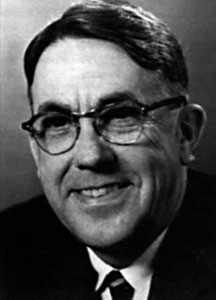
\includegraphics[width = 1.3in]{This_is_the_photo_of_Arthur_Samuel.jpg}
\caption{Arthur Samuel}
\end{figure}

Arthur Lee Samuel (December 5, 1901 – July 29, 1990)was an American pioneer in the field of computer gaming and artificial intelligence.He coined the term "machine learning" in 1959.The Samuel Checkers-playing Program was among the world's first successful self-learning programs, and as such a very early demonstration of the fundamental concept of artificial intelligence (AI).He was also a senior member in the TeX community who devoted much time giving personal attention to the needs of users and wrote an early TeX manual in 1983.

\subsection{Tom Michell's definition}
\large \textbf{A computer program is said to learn from experience E with respect to some task T and some performance measure P,if its performance on T,as measured by P,improves with experience E.}

乍一看这个写的比较拗口,但实际上也就是说通过对experience E的学习,使原有task T的performance P有了提高。对于Tom Michell的了解大概是因为那本机器学习的教材,薄薄一本,当时应该是看过同学的,没有看太多,也不好评价。这个定义就显得更像在描述一个事情而非定义。本书接下来用一个简单的例子来说明了一下,那就是spam filter,并将Tom Michell的定义套用做了讲解。
\begin{figure}[H]
\centering
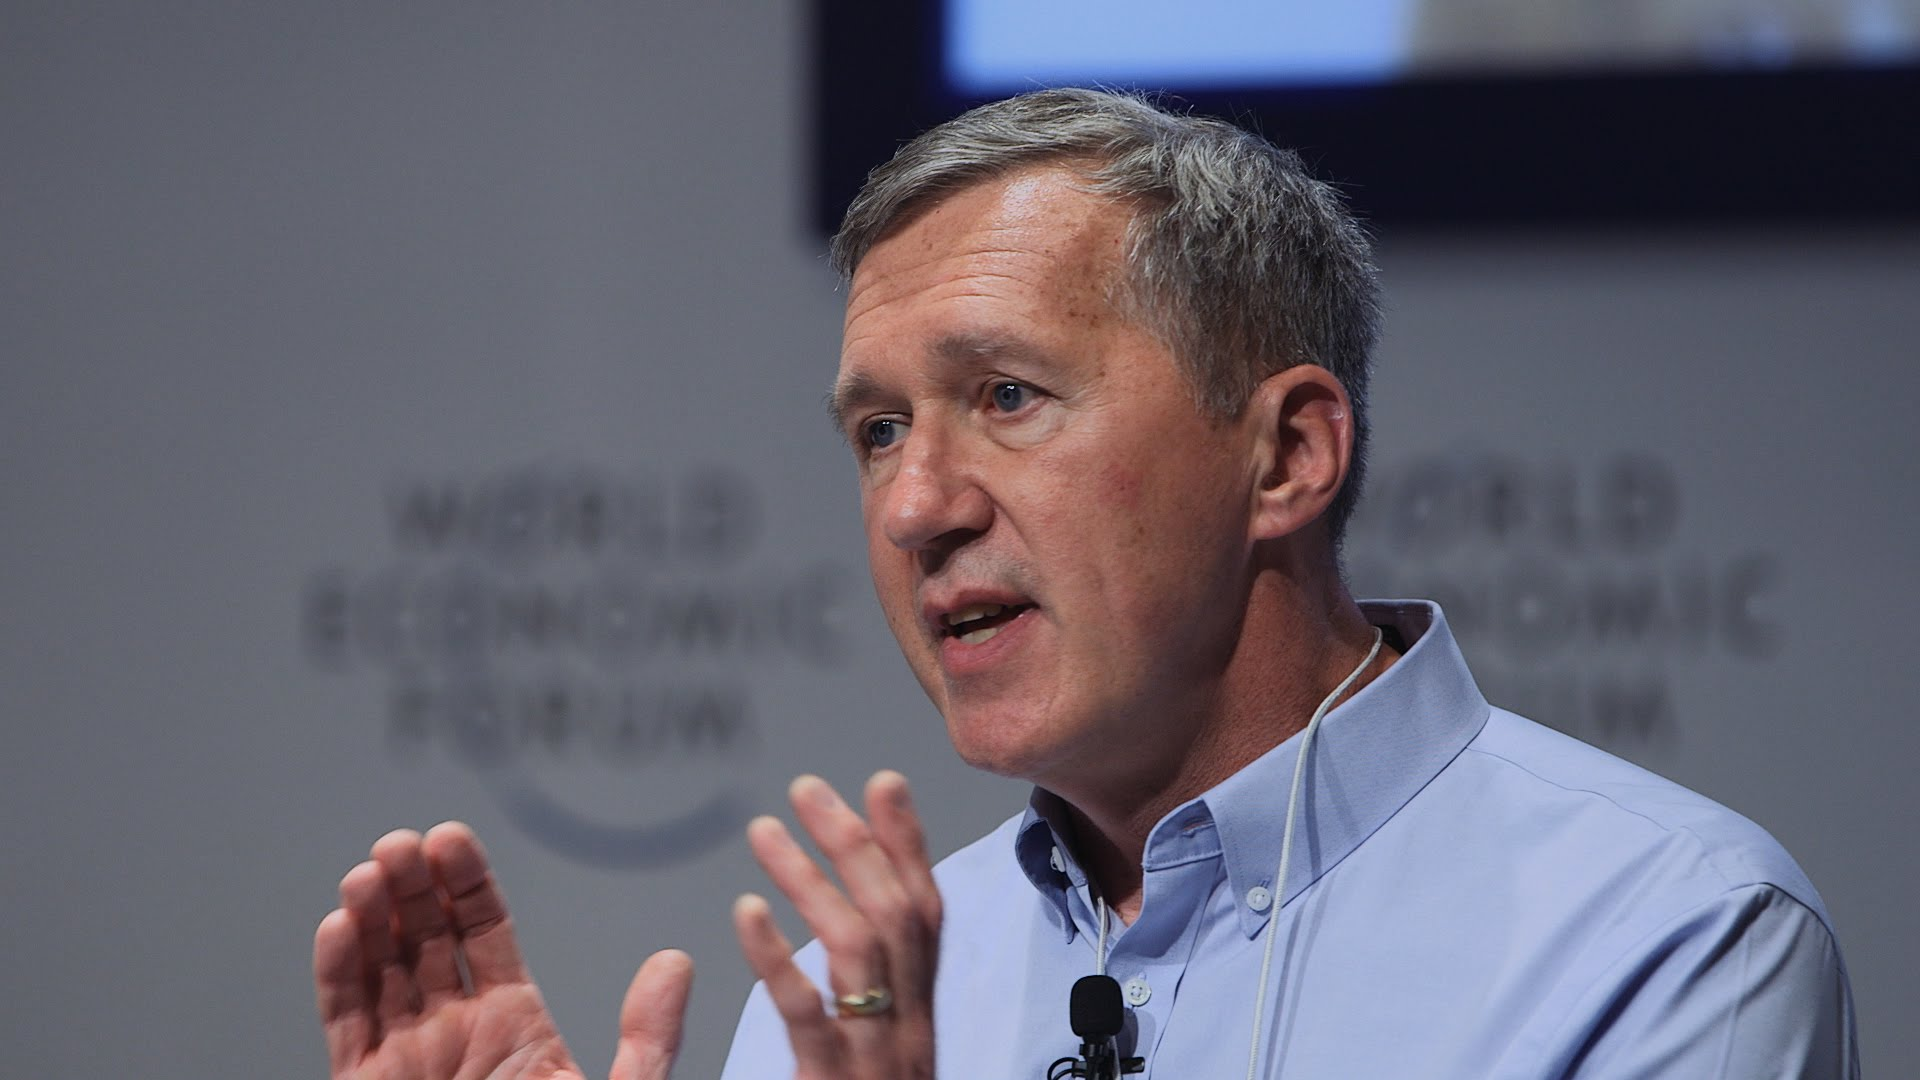
\includegraphics[width = 2in]{TomWEF2017.jpg}
\caption{Tom Michell}
\end{figure}

\section{Why use Machine Learning}
依旧以写一个spam filter为例,当使用传统的编程技术时,需要一个长长的规则清单,并且这个规则是难以把握且复杂的。相反,当使用Machine Learning Techniques时,可以让机器自主的学习知识,学习垃圾邮件中的词频,这显然更加简洁高效。To summarize,Machine Learning is great for:
\begin{enumerate}

\item Problems require a lot of hand-tuning or long list of rules.

\item Complex problems is no good solution using traditional approach.

\item Fluctuating enviornment

\item Getting insights about complex problems and large amount of data
\end{enumerate}

\subsection{Types of Machine Learning Systems}
\begin{itemize}
	\item[-] Whether or not they are trained with human supervision(Supervised Unsupervised Semisupervised Reinforcement Learning 监督 非监督 半监督 强化学习)

	\item[-] Whether or not they can learn incrementally(Online versus Batch learning 在线学习 VS 批量学习)

	\item[-] Whether work by comparing new data to  known data or instead detect patterns in the training data and build a predictive model(instance-based versus model-based learning 基于模型 vs 基于实例)

\end{itemize}

\section{Supervised/Unsupervised Learning}
\subsection{Supervised Learning}

The training data you feed to the algorithm includes the desire solutions,called \emph{labels}.Here are some most important supervised learning algorithms(在后文中都有体现):

\begin{itemize}
	\item[-] k-Nearest Neighbors
	\item[-] Linear Regression
	\item[-] Logistic Regression
	\item[-] Support Vector Machines
	\item[-] Decision Trees and Random Forests
	\item[-] Neural networks
\end{itemize}

\subsection{Unsupervised Learning}

The training data is unlabeled.Some important unsupervised learning algorithms:
\begin{itemize}
	\item Clustering
	\item[-] k-Means
	\item[-] Hierarchical Cluster Analysis(HCA)
	\item[-] Expection Maximization
	\item Visualization and dimensionality reduction
	\item[-] Principle Component Analysis(PCA)
	\item[-] Kernel PCA
	\item[-] Locally-Linear Embedding(LLE)
	\item[-] t-distributed Stochastic Neighbor Embedding(t-SNE)
	\item Associaton rule learning
	\item[-] Apriori
	\item[-] Eclat
\end{itemize}

\subsection{Semisupervised Learning}
Algorithms can deal with partially labeled training data(usually a lot of unlabeled data and a little bit of labeled data) is called semisupervised learning

\subsection{Reinforcement Learning}
Reinforcement learning (RL) is an area of machine learning concerned with how software agents ought to take actions in an environment so as to maximize some notion of cumulative reward. 

\section{Batch and Online Learning}
Whether the system can learn incrementally from a stream of income data or not is the criterion to classify batch learning and online learning.

\subsection{Batch learning}
First the system is trained,and then it is launched into production and runs without learning anymore,it just apply what it has learned,it also called offline learning.

\subsection{Online learning}
In online learning,you train the system incrementally by feeding it data instances sequentially,either individually or by small groups called mini-batches.

\section{Instance-based versus Model-based learning}
Two generalization methods:Instance-based and model-based learning.

\subsection{Instance-based learning}
The system learns the examples by heart,then generalizes to new cases using a similiarity measure.

\subsection{Model-based learning}
Building a model of the examples,then use the model to make predications.The book using a linear regression problem as an example.

\subsection{Training and running a linear model using Scikit-Learn}
在对数据进行处理前,需要先获得数据,本书都使用真实数据来进行处理。第一个程序所用的程序来自OECD(Organisation for Economic Co-Operation and Development)。本书给出的是一个短链接\url{ https://stats.oecd.org/index.aspx?DataSetCode=BLI}可以在网站直接下载每一年的数据。具体的情况大家可以自行下载或者看下图表头。
\begin{figure}[H]
\centering
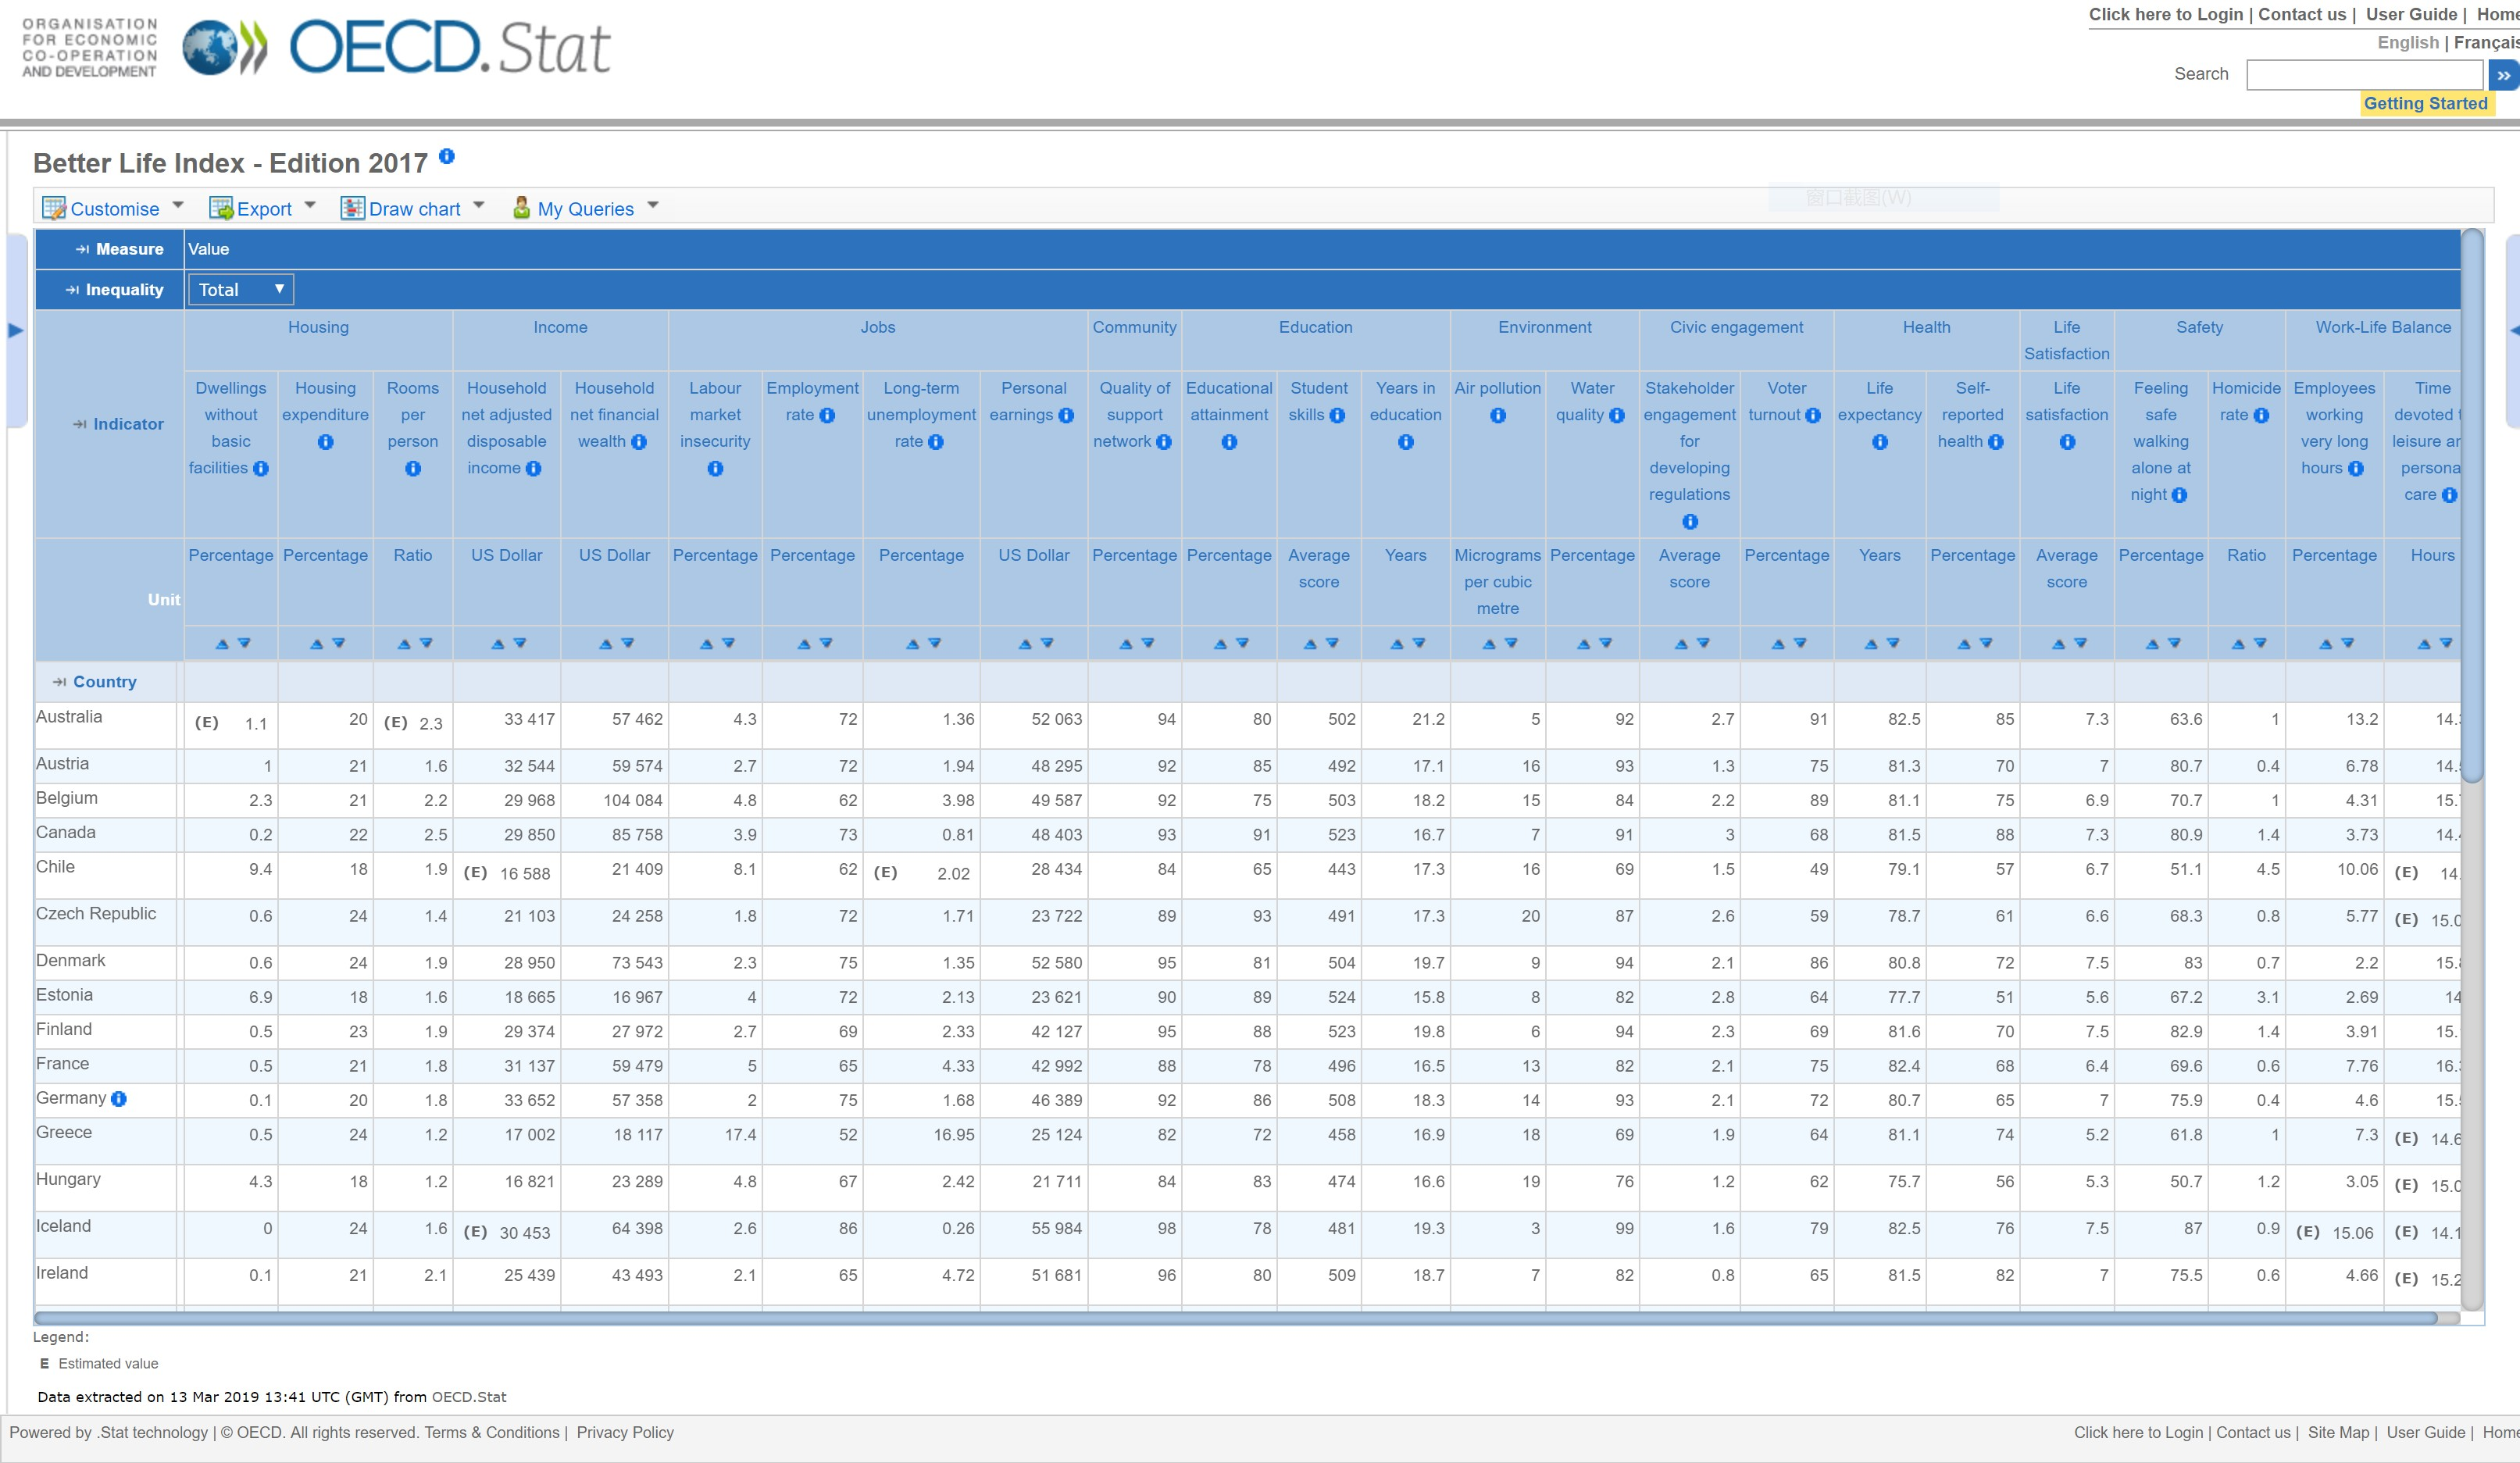
\includegraphics[width = 6in]{oedc.jpg}
\caption{OEDC 网站截图}
\end{figure}


\begin{lstlisting}
import matplotlib
import matplotlib as plt
import numpy as np
import pandas as pd
import sklearn


\end{lstlisting}

\end{document}